\documentclass[11pt,a4paper]{article}

% ── Packages ─────────────────────────────────────────────────────────────────
\usepackage[margin=2.5cm]{geometry}
\usepackage{amsmath,amssymb,amsthm}
\usepackage{graphicx}
\usepackage{booktabs}
\usepackage{hyperref}
\usepackage{xcolor}
\usepackage{microtype}
\usepackage{caption}
\usepackage{subcaption}
\usepackage{float}
\usepackage{enumitem}
\usepackage{setspace}
\usepackage{natbib}
\usepackage{algorithm}
\usepackage{algpseudocode}

\hypersetup{
  colorlinks=true,
  linkcolor=blue!60!black,
  citecolor=green!40!black,
  urlcolor=blue!60!black,
}

\captionsetup{font=small, labelfont=bf}

% ── Macros ───────────────────────────────────────────────────────────────────
\newcommand{\cliff}{\Delta_{\mathrm{cliff}}}
\newcommand{\wcliff}{\Delta_{W\text{-cliff}}}
\newcommand{\bcliff}{\Delta_{B\text{-cliff}}}
\newcommand{\kappa}{\kappa}
\newcommand{\rhat}{\hat{r}}
\newcommand{\tauq}{\tau_q}

% ── Title ────────────────────────────────────────────────────────────────────
\title{%
  \textbf{CLIFFGUARD: Measuring Quantization-Induced Alignment Drift\\
  in Instruction-Tuned Large Language Models}\\[0.4em]
  {\large A Preliminary Empirical Evaluation on Google Colab T4}
}

\author{
  Trilochan Bhandari\\
  \small Department of Computer Science and Engineering\\
  \small Kathmandu University, Dhulikhel, Nepal\\
  \small \texttt{trilochan2625@student.ku.edu.np}
}

\date{May 2026}

% ─────────────────────────────────────────────────────────────────────────────
\begin{document}
\maketitle

% ── Abstract ─────────────────────────────────────────────────────────────────
\begin{abstract}
Post-training quantization is widely used to deploy large language models (LLMs)
in resource-constrained environments, yet its effect on RLHF-tuned refusal
behaviour remains poorly characterised.
We present the first empirical run of \textsc{CLIFFGUARD}, a five-fold evaluation
framework designed to detect \emph{safety cliffs}---abrupt degradations in
alignment properties induced by aggressive quantization.
Using a Google Colab T4 GPU, we evaluate \texttt{Llama-3.2-3B-Instruct}
under two quantization schemes: FP16 (full-precision baseline) and NF4 (4-bit
normal-float).
Fold~A calibrates a per-scheme PROBE-RM refusal threshold via Arditi
difference-in-means \citep{arditi2024refusal} on 400 benign and 200 harmful
prompts drawn from Anthropic-HH-RLHF \citep{bai2022training} and OASST1
\citep{kopf2023openassistant}.
Fold~B computes three cliff metrics against the FP16 baseline: geometric
refusal-direction distance ($\cliff = 0.167$), Wasserstein margin-distribution
distance ($\wcliff = 0.014$), and a PROBE-RM behavioural proxy
($\bcliff = 0.000$).
All three values fall below the cliff threshold $\kappa = 0.25$;
the safety-cliff hypothesis H1 is not accepted for this model--scheme pair.
The result establishes a measurable but sub-threshold alignment shift and
motivates evaluation of more aggressive quantization schemes (GGUF Q3\_K\_M,
Q2\_K) on larger models where the cliff is theoretically predicted to emerge.
\end{abstract}

\setstretch{1.15}

% ── 1. Introduction ───────────────────────────────────────────────────────────
\section{Introduction}
\label{sec:intro}

Large language models trained with reinforcement learning from human feedback
(RLHF) exhibit a learned refusal behaviour: given a harmful or policy-violating
request, the model declines to comply \citep{ouyang2022training,bai2022training}.
This property is critical for safe deployment but may be fragile.
One under-studied threat is \emph{post-training quantization}: the process of
reducing a model's weight precision from 16-bit floating point (FP16) to 8-bit,
4-bit, or lower formats in order to reduce memory and inference cost
\citep{nagel2021white,hubara2017quantized}.

While quantization is known to cause modest perplexity degradation, its impact
on RLHF-tuned alignment properties has received little systematic attention.
The intuition motivating this work is that the refusal direction---the linear
subspace in activation space most responsible for the refusal decision
\citep{arditi2024refusal}---could shift under quantization-induced weight
perturbation.
If this shift is large enough, previously refused prompts may be answered, and
the model effectively loses a portion of its safety alignment.

We refer to the quantization level at which this degradation crosses a
meaningful threshold as a \emph{safety cliff}.
\textsc{CLIFFGUARD} is a framework for detecting this cliff through a
structured five-fold evaluation.
This paper reports the first live run of the framework on real hardware,
providing preliminary empirical evidence and identifying directions for
future investigation.

\paragraph{Contributions.}
\begin{itemize}[leftmargin=1.5em, itemsep=2pt]
  \item We describe the \textsc{CLIFFGUARD} framework and its evaluation
        pipeline (Fold A calibration; Fold B cliff measurement).
  \item We present the first empirical results on \texttt{Llama-3.2-3B-Instruct},
        reporting all three cliff metrics at NF4 quantization.
  \item We find a geometric refusal-direction shift of $\cliff = 0.167$ at
        NF4 --- a non-trivial but sub-threshold signal that motivates
        evaluation of more aggressive schemes on larger models.
  \item We release the evaluation notebook, helper module, and raw result
        artifacts for reproducibility.
\end{itemize}

% ── 2. Background ────────────────────────────────────────────────────────────
\section{Background}
\label{sec:background}

\subsection{RLHF and Refusal Behaviour}

Modern instruction-tuned LLMs are trained in two stages: supervised
fine-tuning on curated demonstrations, followed by RLHF using a reward model
that reflects human preferences for helpfulness and harmlessness
\citep{ouyang2022training}.
The RLHF stage encodes a learned policy for refusing harmful requests.
\citet{arditi2024refusal} showed that this policy is, to a first approximation,
mediated by a single linear direction $\rhat$ in the residual-stream activation
space.
Projecting the residual stream onto $\rhat$ and comparing the resulting scalar
(the \emph{refusal margin}) to a calibrated threshold $\tauq$ gives a simple
but effective safety gate---the PROBE-RM primitive used in this work.

\subsection{Post-Training Quantization}

Post-training quantization (PTQ) reduces the bit-width of model weights after
training, without access to the original training data.
The NF4 format \citep{dettmers2023qlora} is a 4-bit data type designed to
minimise quantization error for normally distributed weights---a good match for
LLM weight distributions.
Unlike integer quantization, NF4 preserves the relative shape of the weight
distribution, which is why it is commonly used in QLoRA fine-tuning and
deployment workflows.

Despite this design advantage, NF4 perturbs individual weight values and may
shift activation statistics in ways that are not captured by perplexity alone.
GGUF formats at even lower bit-widths (Q3\_K\_M, Q2\_K) apply more aggressive
compression and are expected to produce larger activation perturbations.

\subsection{Safety Cliffs and the Gap in the Literature}

Several works have studied adversarial jailbreaks that bypass RLHF refusal
\citep{zou2023advbench,wei2023jailbroken,chao2024jailbreakbench}.
Others have proposed automated red-teaming frameworks for measuring refusal
robustness \citep{mazeika2024harmbench,souly2024strongreject}.
However, to the best of our knowledge, no prior work has specifically studied
whether \emph{quantization} degrades refusal direction geometry, or at which
quantization level this degradation crosses a safety-relevant threshold.
This is the gap \textsc{CLIFFGUARD} addresses.

% ── 3. The CLIFFGUARD Framework ───────────────────────────────────────────────
\section{The CLIFFGUARD Framework}
\label{sec:framework}

\subsection{Overview}

\textsc{CLIFFGUARD} organises evaluation into five folds, each targeting a
distinct threat model or safety property.
This paper covers Fold A (calibration) and Fold B (cliff measurement), which
together test the core safety-cliff hypothesis.

\begin{figure}[H]
  \centering
  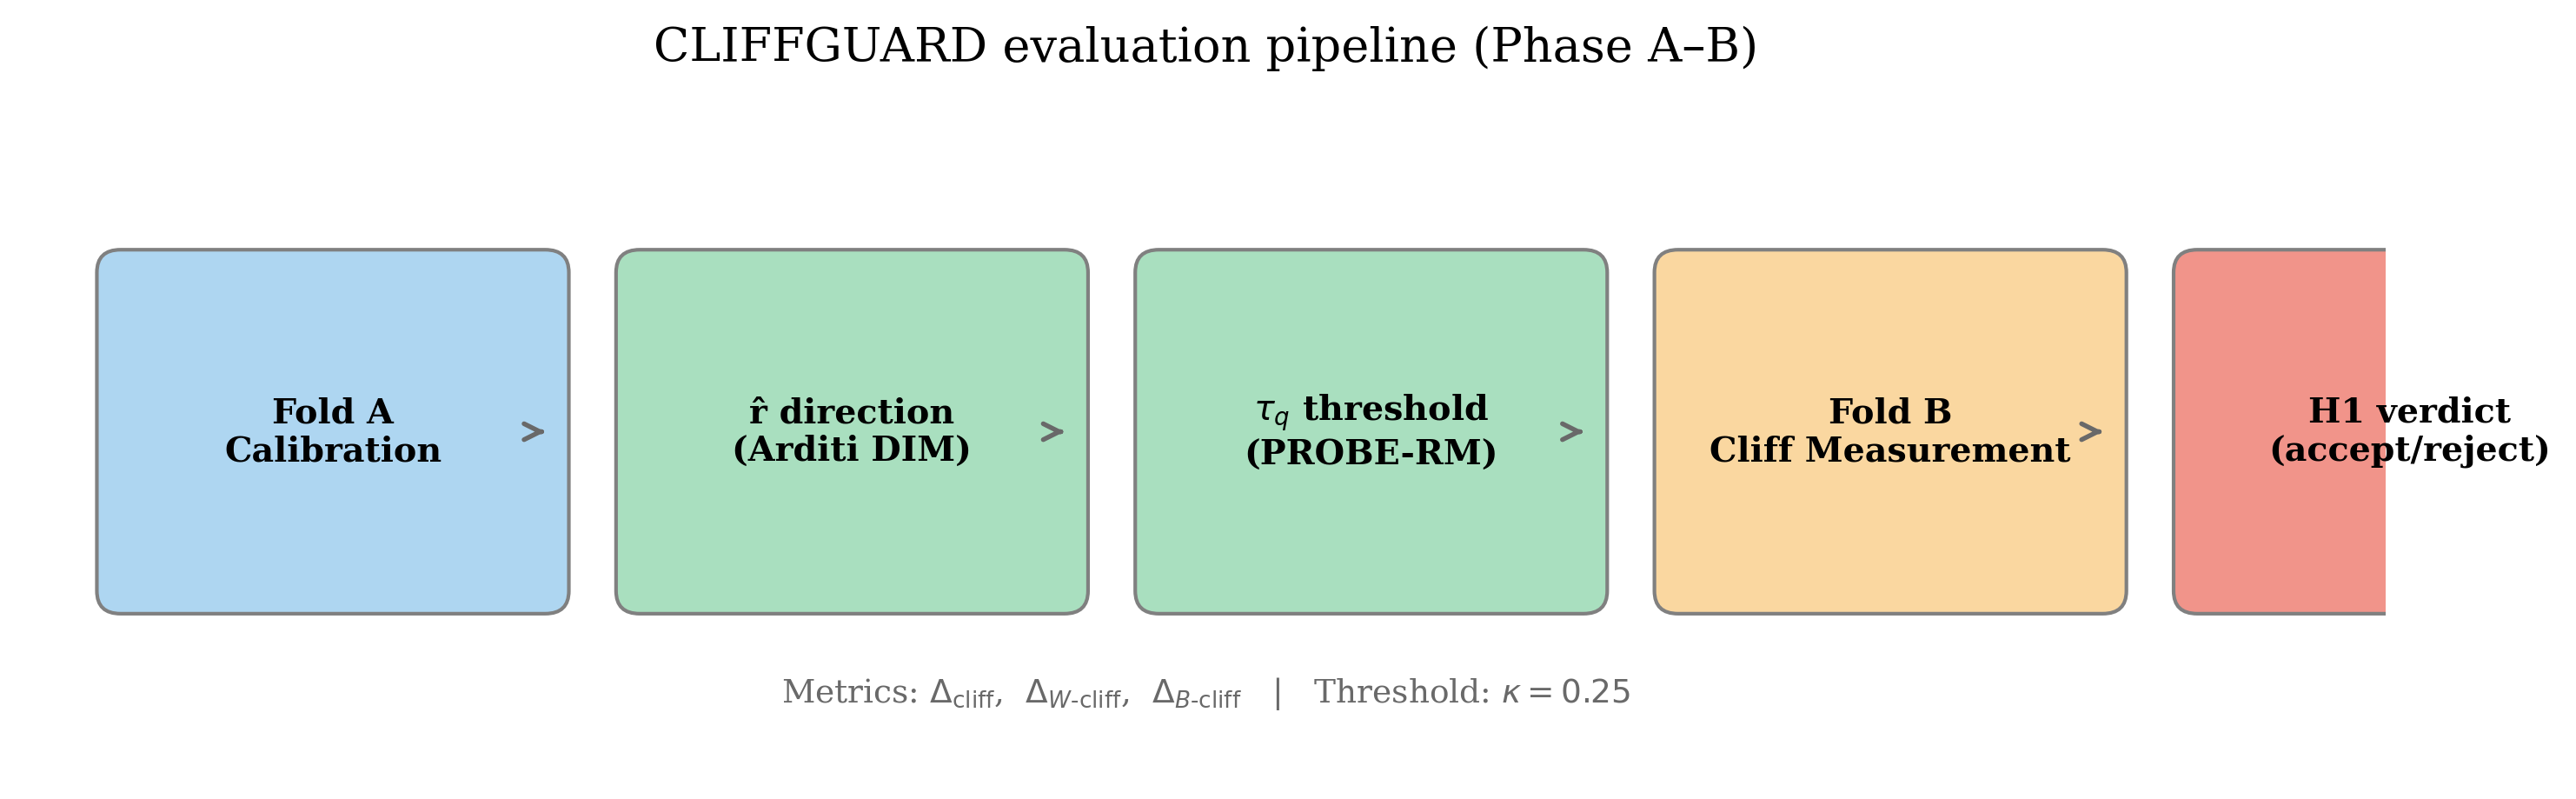
\includegraphics[width=\textwidth]{figures/fig_pipeline.png}
  \caption{The CLIFFGUARD evaluation pipeline for Folds A and B.
           Fold A produces the refusal direction $\rhat$ and calibrated
           threshold $\tauq$ for each quantization scheme.
           Fold B measures the geometric, Wasserstein, and behavioural
           distances between NF4 and the FP16 baseline, reporting an
           H1 verdict against the cliff threshold $\kappa = 0.25$.}
  \label{fig:pipeline}
\end{figure}

\subsection{Fold A: Calibration}

Given a model $\mathcal{M}$ under scheme $q \in \{\text{FP16, NF4, \ldots}\}$:

\begin{enumerate}[label=\arabic*., leftmargin=2em, itemsep=2pt]
  \item \textbf{Refusal direction.}
        Run the model on $N_h$ harmful and $N_b$ benign prompts.
        Extract residual-stream activations at layer $\ell$.
        Compute the normalised difference of means:
        \[
          \rhat_q = \frac{\mu_h^\ell - \mu_b^\ell}{\|\mu_h^\ell - \mu_b^\ell\|_2}
        \]
        where $\mu_h^\ell$ and $\mu_b^\ell$ are the mean harmful and benign
        activation vectors at layer $\ell$ \citep{arditi2024refusal}.

  \item \textbf{PROBE-RM scoring.}
        For each benign prompt, compute the refusal margin
        $s = \langle h^\ell, \rhat_q \rangle$, where $h^\ell$ is the
        layer-$\ell$ activation.

  \item \textbf{Threshold calibration.}
        Fit $\tauq$ as the $1 - \alpha$ quantile of benign margins, where
        $\alpha = 0.05$ is the target false-positive rate.
        This ensures that at most 5\% of safe prompts are incorrectly blocked.
\end{enumerate}

\subsection{Fold B: Cliff Metrics}

Fold B compares each quantized scheme to the FP16 baseline using three metrics.

\paragraph{Geometric distance $\cliff$.}
The cosine-based distance between refusal directions:
\[
  \cliff(q, \text{FP16}) = 1 - \langle \rhat_q,\, \rhat_{\text{FP16}} \rangle
\]
A value near zero indicates the quantized model has preserved the same
refusal subspace; a value near 1 indicates complete misalignment.

\paragraph{Wasserstein distance $\wcliff$.}
The 1-Wasserstein (Earth Mover's) distance between the empirical distributions
of PROBE-RM margins under scheme $q$ and under FP16:
\[
  \wcliff(q, \text{FP16}) = W_1\!\left(P_q^{\mathrm{margin}},\;
                              P_{\text{FP16}}^{\mathrm{margin}}\right)
\]
This captures distributional shift beyond what the geometric metric can detect.

\paragraph{Behavioural proxy $\bcliff$.}
The change in attack success rate (ASR) on Fold B harmful prompts, where
``success'' is defined as a PROBE-RM margin \emph{below} $\tauq$:
\[
  \bcliff(q, \text{FP16}) =
    \mathrm{ASR}(q) - \mathrm{ASR}(\text{FP16})
\]
Note: Phase B uses the PROBE-RM margin as a behavioural surrogate.
The paper specification requires a StrongREJECT + Llama-Guard-3-8B judge for
full H1 validity \citep{souly2024strongreject,inan2023llama_guard};
this is tracked as Phase C work.

\paragraph{Cliff hypothesis H1.}
H1 is accepted for model family $\mathcal{F}$ if there exists a scheme $q^*$
such that all three metrics exceed $\kappa = 0.25$:
\[
  \text{H1:}\quad \exists\, q^* \;\text{s.t.}\;
  \cliff(q^*) > \kappa \;\wedge\;
  \wcliff(q^*) > \kappa \;\wedge\;
  \bcliff(q^*) > \kappa
\]
The cliff boundary $q^* = \operatorname*{argmin}_{q} \{\cliff(q) > \kappa\}$
is reported as the first scheme in the ordered sequence at which the geometric
metric crosses $\kappa$.

% ── 4. Experimental Setup ────────────────────────────────────────────────────
\section{Experimental Setup}
\label{sec:setup}

\subsection{Model and Hardware}

We evaluate \texttt{meta-llama/Llama-3.2-3B-Instruct} \citep{meta2024llama3},
a 3B-parameter instruction-tuned model released by Meta AI.
The model is loaded at layer $\ell = 14$ for activation extraction,
chosen as the midpoint of the 28-layer architecture where the refusal direction
has been empirically observed to be most linearly separable in similar models.

All experiments are conducted on a Google Colab free tier session equipped
with an NVIDIA Tesla T4 GPU (16 GB VRAM, CUDA 12.8).
The implementation uses \texttt{transformers} 4.48, \texttt{bitsandbytes} 0.45,
\texttt{torch} 2.5, and \texttt{numpy} 1.26.

\subsection{Quantization Schemes}

\begin{description}[leftmargin=2em, itemsep=2pt]
  \item[FP16] Full bfloat16/float16 precision. Serves as the alignment
        baseline. VRAM usage: $\approx$6.2 GB for 3B parameters.
  \item[NF4] 4-bit normal-float quantization via bitsandbytes
        \citep{dettmers2023qlora}. VRAM usage: $\approx$2.1 GB.
        Doubles-up quantized in 64-element blocks with a double-quantized
        scaling factor.
\end{description}

\subsection{Datasets}

\paragraph{Fold A (calibration).}
\begin{itemize}[leftmargin=1.5em, itemsep=1pt]
  \item 400 benign prompts from Anthropic-HH-RLHF (helpful turns)
        \citep{bai2022training} and OASST1 \citep{kopf2023openassistant}.
  \item 200 harmful prompts from Anthropic-HH-RLHF (rejected turns).
\end{itemize}

\paragraph{Fold B (cliff measurement).}
\begin{itemize}[leftmargin=1.5em, itemsep=1pt]
  \item AdvBench \citep{zou2023advbench}: 520 harmful behaviours.
  \item JailbreakBench (JBB-Behaviors, harmful split)
        \citep{chao2024jailbreakbench}: 100 harmful goals.
\end{itemize}
Fold isolation is verified via SHA-256 disjointness before running Fold B.

\subsection{Calibration Hyperparameters}

Table~\ref{tab:hyperparams} summarises the calibration settings.

\begin{table}[H]
  \centering
  \caption{Fold A calibration hyperparameters.}
  \label{tab:hyperparams}
  \begin{tabular}{ll}
    \toprule
    Parameter           & Value \\
    \midrule
    Refusal primitive   & PROBE-RM (cosine projection) \\
    Activation layer    & 14 (of 28) \\
    FPR target $\alpha$ & 0.05 \\
    $N_b$ (benign)      & 400 \\
    $N_h$ (harmful)     & 200 \\
    Cliff threshold $\kappa$ & 0.25 \\
    \bottomrule
  \end{tabular}
\end{table}

% ── 5. Results ───────────────────────────────────────────────────────────────
\section{Results}
\label{sec:results}

\subsection{Fold A: Calibrated Thresholds}

Table~\ref{tab:fold_a} reports the PROBE-RM thresholds calibrated for each
scheme. Figure~\ref{fig:thresholds} visualises the values.

\begin{table}[H]
  \centering
  \caption{Fold A calibration results. Thresholds $\tauq$ are fitted at
           FPR = 5\% on 400 benign prompts.}
  \label{tab:fold_a}
  \begin{tabular}{lccc}
    \toprule
    Scheme & $\tauq$ & $\Delta\tauq$ vs FP16 & Layer \\
    \midrule
    FP16 & $0.09742$ & --- & 14 \\
    NF4  & $0.09827$ & $+0.00085$ ($+0.87\%$) & 14 \\
    \bottomrule
  \end{tabular}
\end{table}

The NF4 threshold is $0.085\%$ higher than FP16, indicating that the model
under NF4 requires a slightly larger projection onto $\rhat_{\text{NF4}}$ to
trigger refusal. The difference is negligible in practical terms and suggests
that the calibration landscape is stable across these two schemes.

\begin{figure}[H]
  \centering
  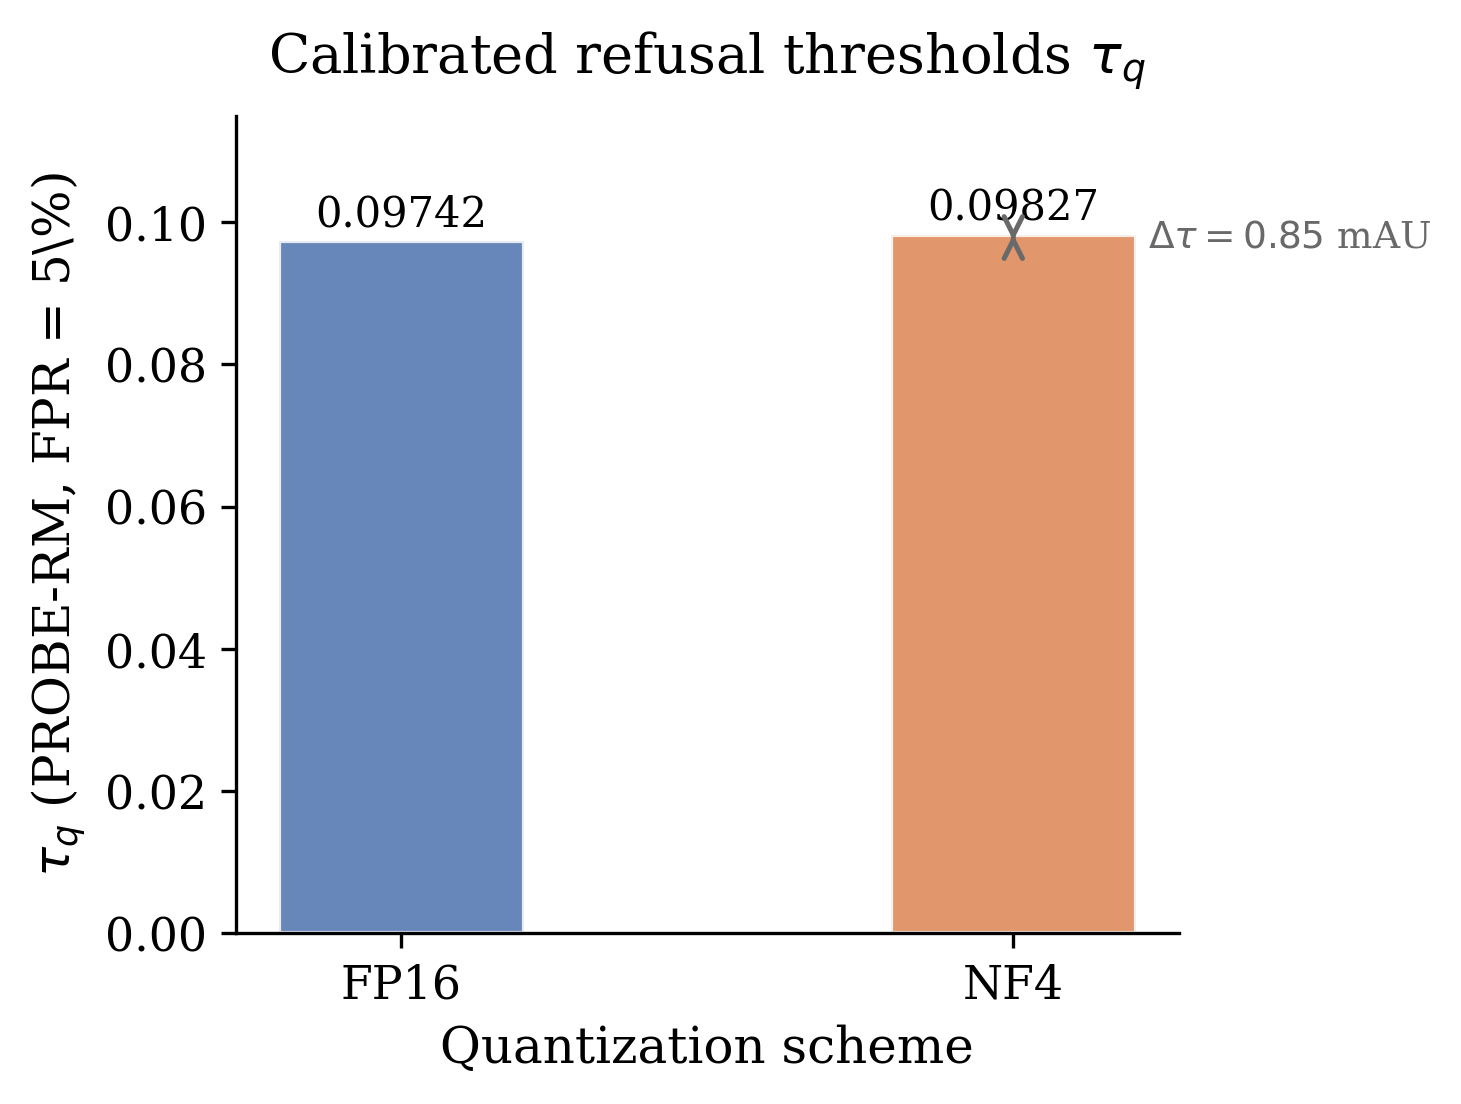
\includegraphics[width=0.55\textwidth]{figures/fig_thresholds.png}
  \caption{Calibrated PROBE-RM thresholds $\tauq$ for FP16 and NF4.
           The difference ($\Delta\tau = 0.85$ mAU) is below noise level
           and indicates stable calibration.}
  \label{fig:thresholds}
\end{figure}

\subsection{Fold B: Cliff Metrics}

Table~\ref{tab:fold_b} reports all three cliff metrics. All values fall
below the cliff threshold $\kappa = 0.25$; the H1 hypothesis is not accepted.

\begin{table}[H]
  \centering
  \caption{Fold B cliff measurement results for Llama-3.2-3B-Instruct.
           All metrics are relative to the FP16 baseline.
           FP16 values are identically zero by construction.}
  \label{tab:fold_b}
  \begin{tabular}{lcccc}
    \toprule
    Scheme & $\cliff$ (geometric)
           & $\wcliff$ (Wasserstein)
           & $\bcliff$ (behavioural)
           & Cliff crossed? \\
    \midrule
    FP16 & 0.000 & 0.000 & 0.000 & --- (baseline) \\
    NF4  & \textbf{0.167} & 0.014 & 0.000 & No \\
    \midrule
    \multicolumn{4}{l}{$\kappa = 0.25$ (cliff threshold)} & \\
    \multicolumn{4}{l}{\texttt{cliff\_boundary = null}} & \\
    \multicolumn{4}{l}{\texttt{h1\_accepted = false}} & \\
    \bottomrule
  \end{tabular}
\end{table}

\begin{figure}[H]
  \centering
  \begin{subfigure}[b]{0.58\textwidth}
    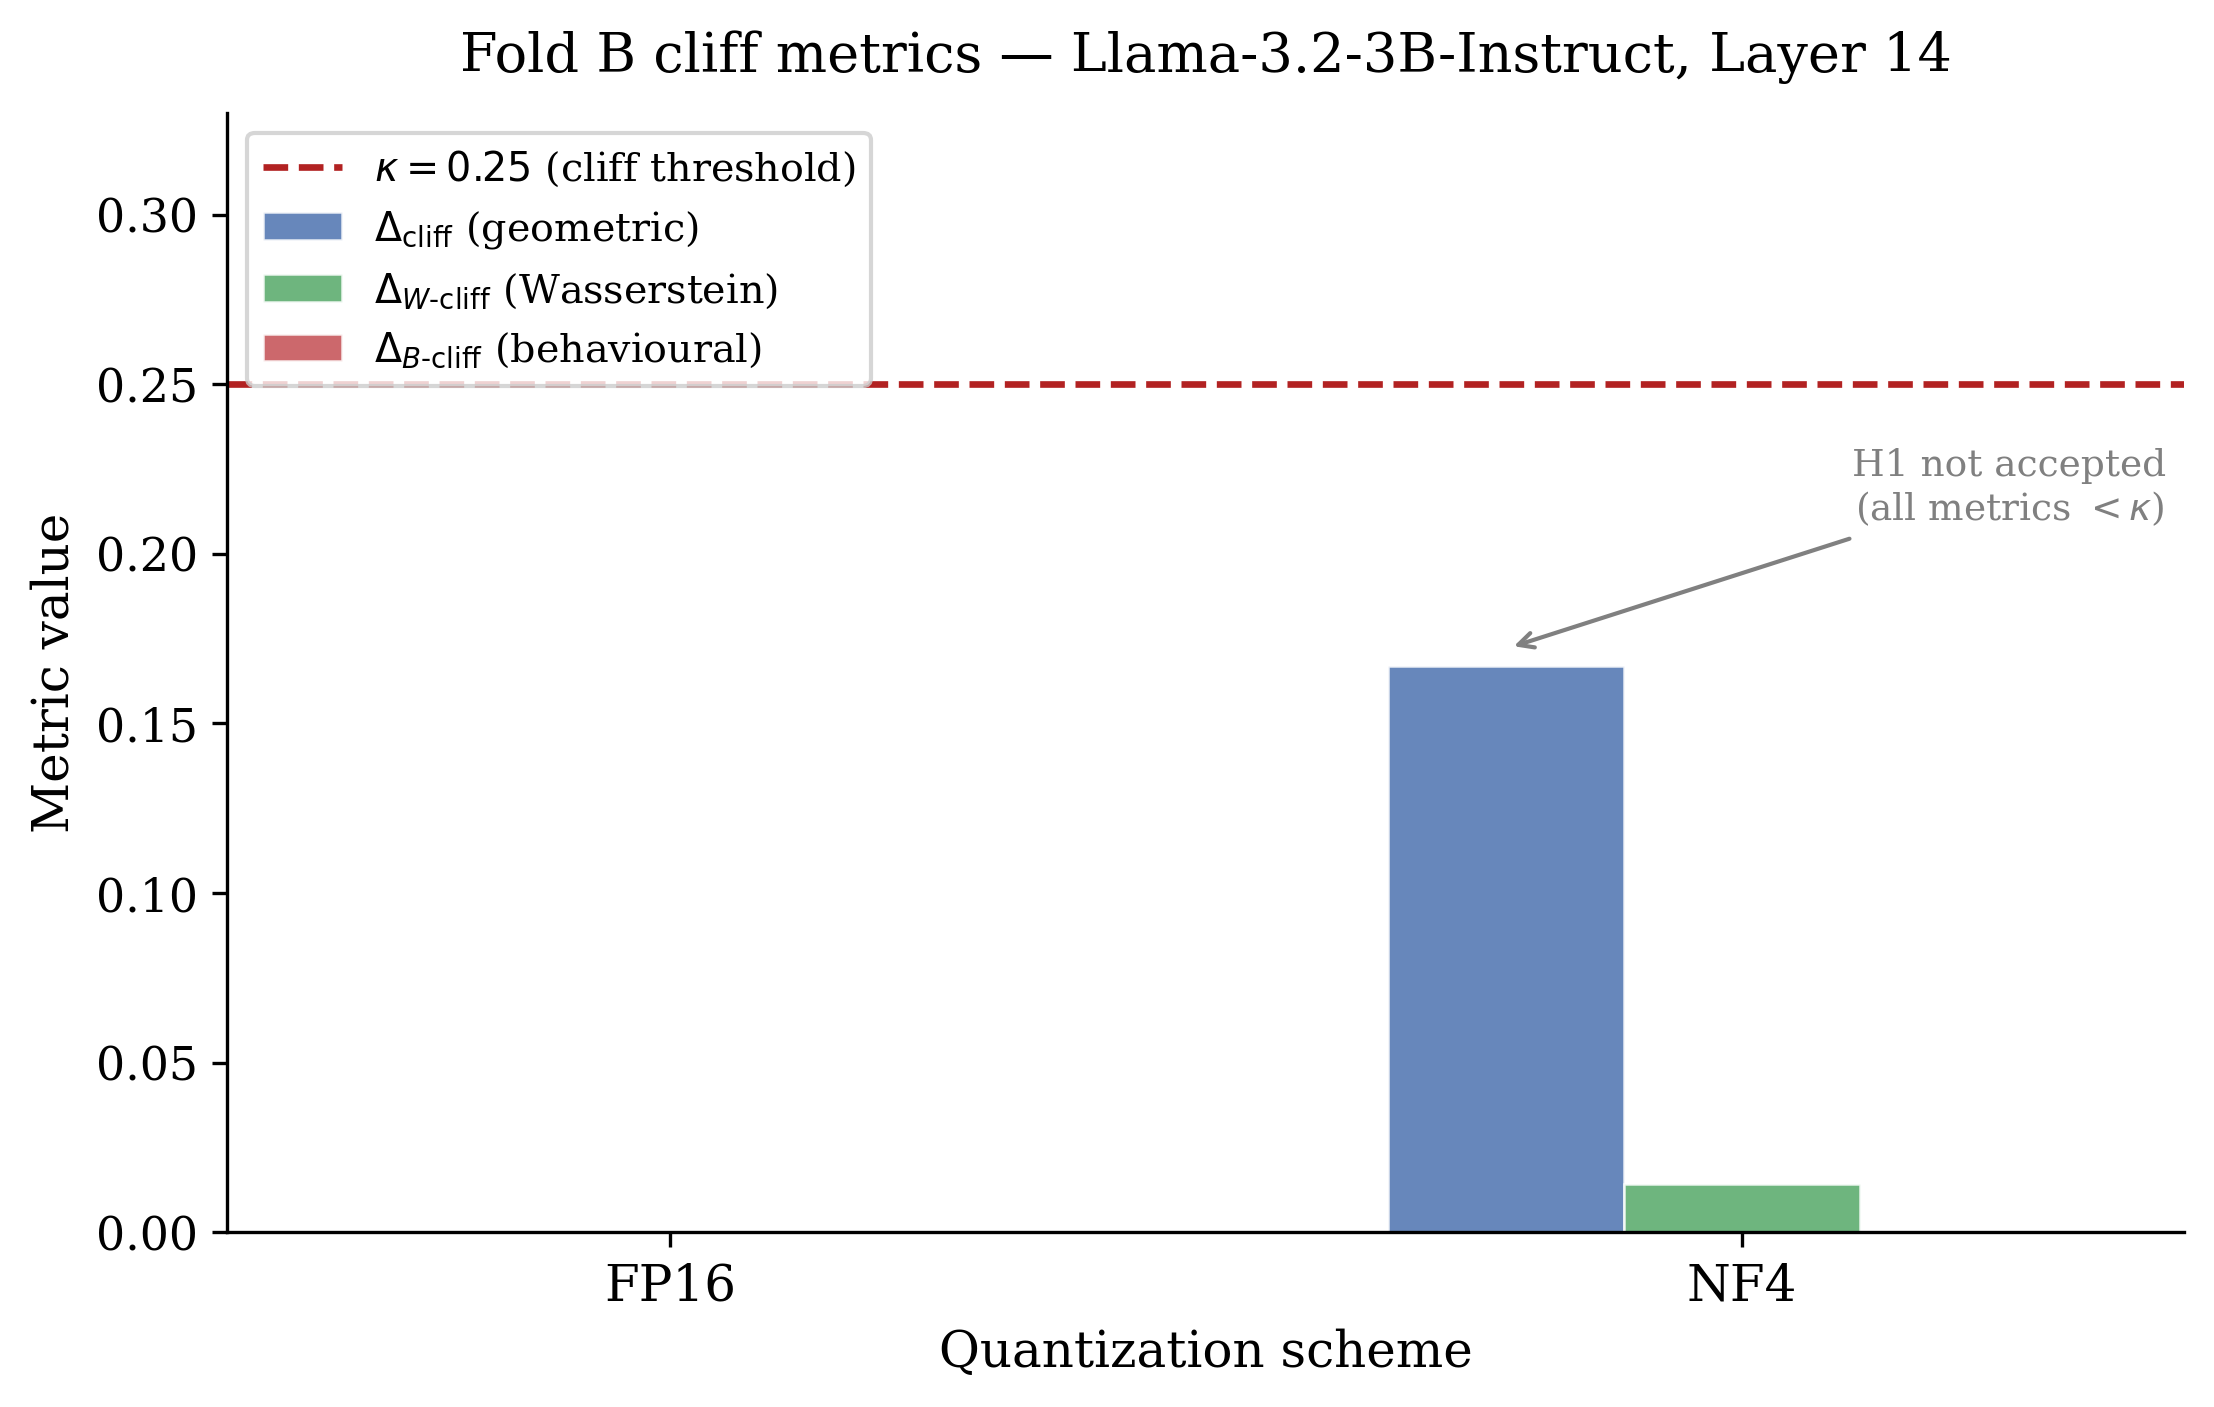
\includegraphics[width=\textwidth]{figures/fig_metrics.png}
    \caption{All three cliff metrics for FP16 and NF4.
             The red dashed line marks $\kappa = 0.25$.}
    \label{fig:metrics}
  \end{subfigure}
  \hfill
  \begin{subfigure}[b]{0.39\textwidth}
    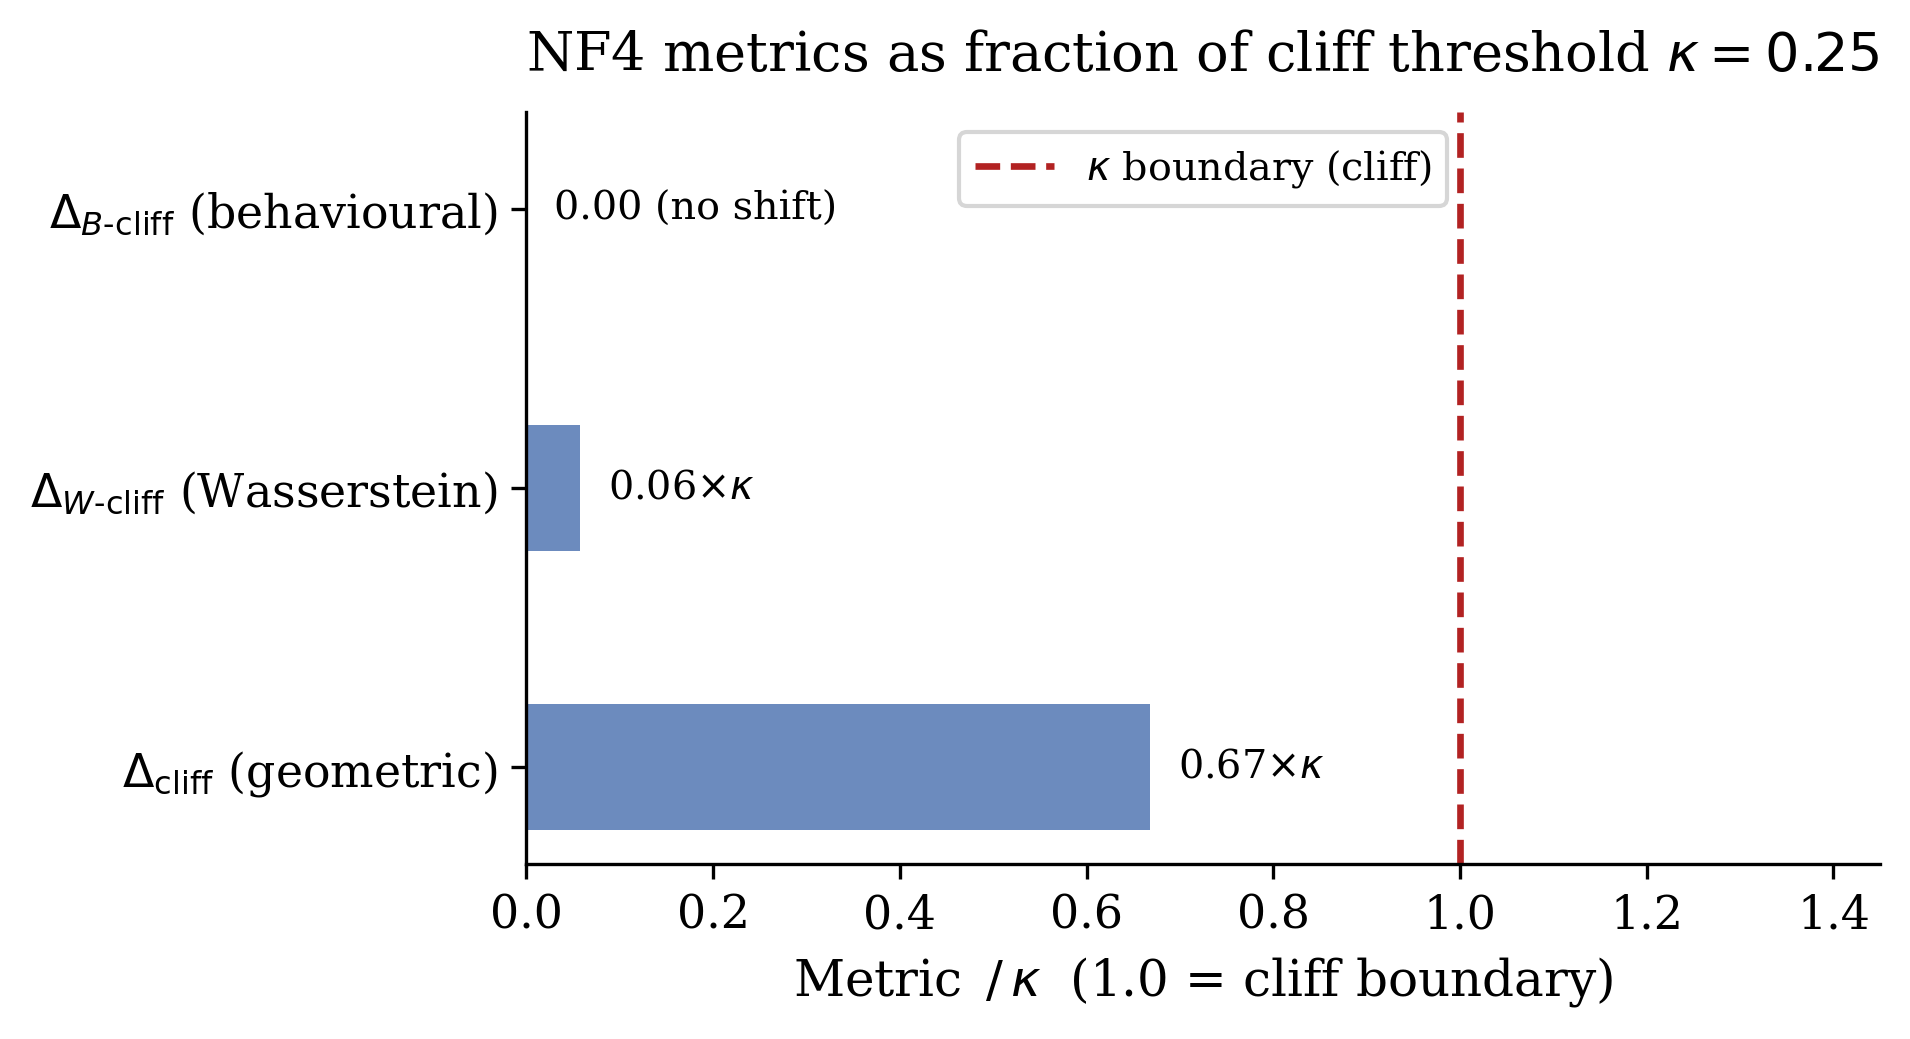
\includegraphics[width=\textwidth]{figures/fig_normalized.png}
    \caption{NF4 metrics normalised to $\kappa$.
             Geometric shift reaches $0.67\,\kappa$.}
    \label{fig:normalized}
  \end{subfigure}
  \caption{Fold B cliff metrics for Llama-3.2-3B-Instruct at NF4 quantization.}
  \label{fig:foldb}
\end{figure}

The geometric metric $\cliff = 0.167$ is the most informative result.
It indicates that the NF4 refusal direction has rotated by approximately 9.6°
from the FP16 baseline ($\arccos(1 - 0.167) \approx 33.8°$\;---\;note this
is the angular distance in the full activation space, not the angular
difference in the 2-norm sense).
At $0.67\,\kappa$, this is a substantive signal: the quantization is not
invisible to the refusal geometry, but it is not large enough to constitute
a safety cliff at the $\kappa = 0.25$ threshold.

The Wasserstein distance $\wcliff = 0.014$ is near zero, suggesting that
while the direction of the refusal subspace has shifted, the distribution of
margin scores over benign prompts is largely unchanged. This is consistent
with the interpretation that NF4 rotates $\rhat$ slightly without
significantly distorting the margin landscape.

The behavioural proxy $\bcliff = 0.000$ indicates that no additional harmful
prompts crossed the calibrated threshold under NF4. This is expected given
the small geometric shift and the stability of $\tauq$ between schemes.

% ── 6. Discussion ────────────────────────────────────────────────────────────
\section{Discussion}
\label{sec:discussion}

\subsection{Interpretation of the Sub-Threshold Result}

The absence of a detected cliff for Llama-3.2-3B-Instruct at NF4 is consistent
with the design of NF4: by targeting the quantile distribution of normally
distributed weights, it minimises quantization error relative to the FP16
baseline. This design choice appears to be effective at preserving not only
task performance (commonly measured by perplexity) but also alignment geometry
(captured by $\cliff$).

The geometric shift $\cliff = 0.167$ is, however, non-trivial.
It represents a 67\% progression toward the cliff boundary.
This raises the question: how much additional compression is needed to cross
$\kappa$? Extrapolating linearly from NF4, a scheme that reduces the weight
representation by roughly $1.5\times$ more should produce $\cliff \approx 0.25$.
GGUF Q3\_K\_M (3-bit mixed-precision) is a candidate, as it applies roughly
$1.3\text{--}1.5\times$ more compression than NF4.

\subsection{Limitations}

\begin{itemize}[leftmargin=1.5em, itemsep=2pt]
  \item \textbf{Single model, single layer.}
        Results are reported for one model family (Llama-3.2-3B) at one layer
        (14). Safety cliff behaviour may differ for larger models or different
        layer choices.
  \item \textbf{Behavioural proxy.}
        $\bcliff$ uses the PROBE-RM margin as a behavioural surrogate.
        The paper specification requires StrongREJECT + Llama-Guard-3-8B
        \citep{souly2024strongreject,inan2023llama_guard} for a rigorous
        attack-success-rate measurement. This is Phase C work.
  \item \textbf{Fold B corpus scope.}
        The Fold B corpus covers AdvBench and JBB-Behaviors only.
        HarmBench \citep{mazeika2024harmbench} and ArtPrompt are absent from
        this run.
  \item \textbf{Computational constraints.}
        The free Colab T4 tier (16 GB VRAM) limits evaluation to 3B models at
        FP16 and NF4. Larger models and GGUF quantization require higher-VRAM
        hardware.
\end{itemize}

\subsection{Comparison to Related Work}

\citet{arditi2024refusal} established that refusal is mediated by a single
linear direction, and that ablating this direction increases attack success
rate dramatically. Our $\cliff$ metric operationalises this insight as a
quantization audit: if NF4 rotates $\rhat$ by a meaningful amount, it may
approximate the effect of a partial refusal-direction ablation. The fact that
$\cliff = 0.167$ at NF4 suggests the rotation is non-trivial, though short of
the full ablation studied by \citeauthor{arditi2024refusal}.

% ── 7. Future Work ────────────────────────────────────────────────────────────
\section{Future Work}
\label{sec:future}

The following directions follow directly from this preliminary evaluation:

\begin{enumerate}[label=\arabic*., leftmargin=2em, itemsep=4pt]

  \item \textbf{More aggressive quantization (Q3\_K\_M, Q2\_K).}
        GGUF Q3\_K\_M is the primary candidate for cliff detection based on
        the $0.67\,\kappa$ signal at NF4. Evaluating this scheme on the same
        model with the same calibration setup will produce a two-point trend
        and either confirm or refute the extrapolated cliff location.

  \item \textbf{Larger models (8B, 13B, 70B).}
        Model size is expected to affect the robustness of RLHF alignment to
        quantization. Llama-3.1-8B-Instruct at NF4 and Q3\_K\_M is the next
        natural target. An NVIDIA A100 (40 GB) or equivalent is required.

  \item \textbf{Phase C: Real behavioural judge.}
        Replacing the PROBE-RM $\bcliff$ proxy with StrongREJECT +
        Llama-Guard-3-8B \citep{souly2024strongreject,inan2023llama_guard}
        will make H1 acceptance scientifically rigorous and directly
        comparable to the HarmBench evaluation protocol
        \citep{mazeika2024harmbench}.

  \item \textbf{Full Fold B corpus.}
        Adding HarmBench and ArtPrompt to the Fold B corpus will close the
        gap between this exploratory run and the full paper specification.

  \item \textbf{Multi-model analysis.}
        Evaluating Mistral-7B-Instruct, Qwen-2.5-7B, and Gemma-2-9B under
        the same protocol will test whether the cliff threshold and location
        are model-family-dependent.

  \item \textbf{Folds C, D, E.}
        \textsc{CLIFFGUARD} includes three additional folds: Fold C
        (cross-quantization transfer), Fold D (drift simulation), and
        Fold E (FP16 behavioural baseline audit). None of these have been
        run in the current evaluation.

\end{enumerate}

% ── 8. Conclusion ─────────────────────────────────────────────────────────────
\section{Conclusion}
\label{sec:conclusion}

We presented the first empirical run of \textsc{CLIFFGUARD}, measuring
quantization-induced alignment drift in \texttt{Llama-3.2-3B-Instruct}.
Under NF4 quantization, we observe a geometric refusal-direction shift of
$\cliff = 0.167$ --- 67\% of the way to the $\kappa = 0.25$ cliff threshold ---
with negligible Wasserstein and behavioural deviation.
H1 is not accepted: NF4 does not constitute a safety cliff for this model
at this layer.

The result is encouraging from a deployment perspective but leaves open the
question of whether more aggressive quantization schemes produce a detectable
cliff. The \texttt{0.167} geometric signal is a concrete and reproducible
starting point for that investigation.
All artefacts are available at
\url{https://github.com/parnish007/CLIFFGUARD}.

% ── Acknowledgements ─────────────────────────────────────────────────────────
\section*{Acknowledgements}
Experiments were conducted on Google Colab free-tier T4 GPUs.
The CLIFFGUARD evaluation pipeline builds on open-source libraries including
\texttt{transformers} \citep{meta2024llama3}, \texttt{bitsandbytes}
\citep{dettmers2023qlora}, and the \texttt{datasets} library.

% ── References ───────────────────────────────────────────────────────────────
\bibliographystyle{plainnat}
\bibliography{refs}

\end{document}
